% CREATE DOCUMENT TYPE
\documentclass{article}

% CALL PACKAGES
\usepackage{graphicx} % Required for inserting images
\usepackage{fancyhdr}
\usepackage{titling}
\usepackage{setspace}
\usepackage{hyperref}
\usepackage{cleveref}
\usepackage{wrapfig}


% HEADER SETTINGS
\pagestyle{fancy} 
\fancyhf{}
\renewcommand{\headrulewidth}{0pt}

% TITLE
\title{Developing low-cost remote sensing systems for survey and monitoring of coastal environments}
\author{Marcel Rodriguez-Riccelli}
\date{\today} 

% FIGURE CAPTION FORMATTING
\usepackage[font=small,labelfont=bf]{caption}

% INDENT SETTINGS
\setlength{\parindent}{15pt} 

% BEGIN DOCUMENT
\begin{document}

% COVER PAGE
\begin{center}
\thispagestyle{empty}
\par{UNIVERSITY OF CALIFORNIA \\[.5cm] Santa Barbara} 
\vspace{1.25cm}
\par{\huge \thetitle}
\vspace{1.5cm}
\par{A Thesis submitted in partial satisfaction of the requirements \\ for the degree Master of Science in Media Arts and Technology}
\vspace{1cm}
{by \par}
\vspace{1cm}
{\theauthor}
\vspace{1.5cm}
\par{Committee in charge:}
\vspace{1cm}
\par{Marko Peljhan}
\vspace{1cm}
\par{Yon Visell}
\vspace{1cm}
\par{Curtis Roads}
\vspace{2cm}
\par{\thedate}
\end{center}

% SIGNATURE PAGE
\newpage
\thispagestyle{empty}
\begin{center}
\par{The thesis of Marcel Rodriguez-Riccelli is approved.}
\vspace{2cm}
\par{\makebox[10cm][l]{\rule{10cm}{0.4pt}}\\
\makebox[10cm][l]{\textit{Marko Peljhan}}}
\vspace{1cm}
\par{\makebox[10cm][l]{\rule{10cm}{0.4pt}}\\
\makebox[10cm][l]{\textit{Yon Visell}}}
\vspace{1cm}
\par{\makebox[10cm][l]{\rule{10cm}{0.4pt}}\\
\makebox[10cm][l]{\textit{Curtis Roads}}}
\vspace{2cm}
\par{\thedate}
\end{center}

% ABSTRACT
\newpage
\fancyhead[C]{ABSTRACT}
\begin{center}
\vspace{1cm}
\par{\thetitle}
\vspace{1cm}
\par{by}
\vspace{1cm}
\par{\theauthor}
\vspace{1cm}
\end{center}
\doublespacing

\par{It is of no coincidence that most of the world's megacities are situated in the coastal zone: the coasts that bound Earth’s oceans have played a pivotal role in human habitation since its advent, by serving as a source of food and energy resources, a gateway for commerce, transportation, and exploration, and host to industrial, defense, and recreational infrastructure. Throughout history, humanity's most prolific polymaths such as Plato, Aristotle, Galileo Galilei, René Descartes, Issac Newton, Daniel Bernoulli, and Pierre-Simon Laplace, have sought to explain marine and coastal phenomenon. The coupling of our understanding of the coastal area to the development of our civilization extends into the modern era, as populations inhabiting coastal zones continue to grow, and warming global climates exacerbate our vulnerability to damaging coastal processes during episodic events such as storm-surges and through gradual changes such as erosion and sea level rise.}

\par{For this reason, a primary goal of coastal science has become the understanding, characterization, and prediction of these dynamic processes. Modeling and mapping coastal features and processes can inform a wide array of applications, including coastal engineering and management, infrastructure planning, fishery maintenance, ecological protection and restoration, and navigation. Achieving accurate models and maps that embed the spatio-temporal dynamism of coastal systems requires broader sensor networks capable of more frequent data sampling. However, the inherent instability of coastal environments often renders long-term in situ data collection difficult, necessitating the use of remote sensing techniques. In previous decades, the high cost and technical complexity of deploying professional-grade remote sensing equipment limited the scope of data collection. Today, advances in technologies—such as sensor miniaturization, improved embedded computing, expanded satellite coverage, and enhanced GPS accuracy, have enabled the development of low-cost survey systems capable of achieving professional-grade resolution and precision. The unique challenges of collecting scientifically robust data from coastal environments demand a cross-disciplinary approach to developing effective and compliant sensing systems.}

\par{Our goal is to aggregate cross-disciplinary knowledge and modern practices that pertain to remote sensing of coastal environments for oceanographic, hydrological, geological, and ecological field research, and to provide a framework for developing bespoke, low-cost, integrated remote sensing systems.}

\par{In the first section, we detail the various hydrological, morphological, ecological, and anthropological processes associated with coastal environments. In the second section, we outline environmental parameters that can be measured using current remote sensing technologies, along with workflows for data collection, aggregation, processing, and application, ensuring compliance with regulatory accuracy standards. Lastly, in the third section, we present examples of low-cost remote sensing systems for coastal survey that we have developed.} 

\fancyhead[C]{ABSTRACT}
\thispagestyle{fancy}

% TABLE OF CONTENTS
\newpage
\fancyhead[C]{TABLE OF CONTENTS}
\thispagestyle{fancy}
\begin{enumerate}
    \item{Coastal processes}
    \begin{enumerate}
        \item{Hydrological}
        \item{Morphological}
        \item{Ecological}
        \item{Anthropological}
    \end{enumerate}

    \item{Survey, preparation, and application}
    \begin{enumerate}
        \item{Environmental parameters}
        \item{Surface models}
        \item{Process models}
        \item{Local population}
    \end{enumerate}

    \item Proposed solutions
    \begin{enumerate}
        \item{Survey pole with MBES \& dual antenna GPS}
        \item{Large quadrotor for bathymetric LiDAR}
        \item{Miniature quadrotor}
        \item{Virtual drone development platform}
    \end{enumerate}

    \item{References}
    \item{Appendix}
\end{enumerate}

% THE NEARSHORE
\newpage
\fancyhead[C]{COASTAL PROCESSES}
\fancyfoot[C]{\thepage} 
\thispagestyle{fancy}
\setcounter{page}{1}

\section{Coastal processes}
\par{\hspace{.5cm}Broadly, a coast is the greater zone extending both landward and seaward from the shoreline (where ocean meets land). There exist several definitions on the extent of the coastal area offered by disparate scientific bodies. Some sources define the coastal zone according to the distance from the shoreline~\textsuperscript{[1]} while others define coasts by the extent of processes which occur as a result of the interface of land and sea.~\textsuperscript{[2]} Within these general differences lie more specific ones: for the former, regulatory bodies from different countries may demarcate the shoreline according to different tidal reference lines.~\textsuperscript{[3]} For the later, practitioners from different fields may include or exclude certain processes from their definition as necessary based on the timescale of the process of interest.~\textsuperscript{[2]}}

\par{The nebulousness of definitions for the coast are a cause of the morphodynamic nature of the area. Hydrodynamic processes occurring at different timescales work simultaneously to continuously transform coasts over time: from short-term transport of sediment caused by local cross-shore wave set-up, to long term eustatic sea level changes which redefine global shorelines and ocean basins from factors such as glaciation and plate tectonics. The importance of these distinctions is manifested in the outcomes for predictive models of coastal morphology: models with strongly embedded equilibrium concepts a have been successful in predicting short-to-medium term (days-to-years) phenomenon than those which occur over long (multi-decadal) timescales.~\textsuperscript{[4]} Coastal managers, scientists, and engineers, have long sought to develop methodologies for predicting shoreline change by modeling these various hydrological processes.~\textsuperscript{[5]} In adherence with the goal of developing remote sensing solutions to sample environmental parameters for a duration most likely limited by the usual time constraints of a scientific research project, for the purposes of this project, we'll define the coast as the area where sub-decadal oceanic processes serve as a factor in influencing local morphology through sediment transport.}

\begin{figure}
    \centering
    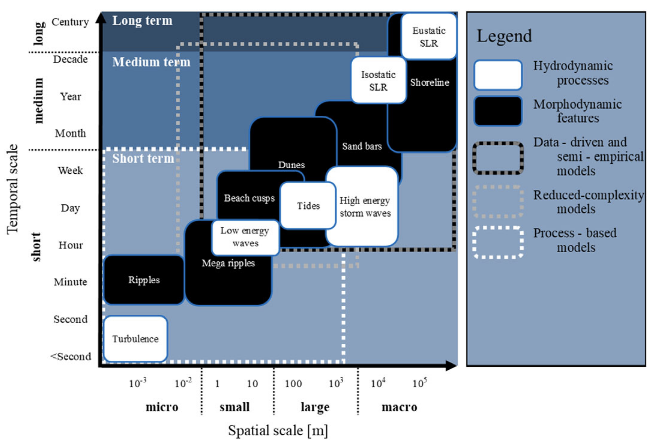
\includegraphics[width=0.8\linewidth]{images/spatial-and-temporal.png}
    \caption{A schematic diagram representing approximate spatial and temporal modelling scales that are appropriate to hydrodynamic processes (white box) and morphodynamic features (black box). Reproduced from Hunt et al. (2023) \textsuperscript{[5]}}
    \label{figure1}
\end{figure}

\par{Sedimentary erosion and accretion caused by hydrological processes derived from waves generated by wind blowing over large stretches of ocean is the predominant morphological influence on most coastal areas.~\textsuperscript{[5]}~\textsuperscript{[6]} As waves are generated over large fetches of ocean and propagate into the nearshore domain (the subaqueous zone commonly spanning 100m directly seaward of the shoreline) they dissipate as depth decreases to beneath their height or they reach the shore. Their energy is augmented by that of other hydrological processes occurring at different spatial and time scales such as tides, to dictate an overall circulatory and sedimentary gradient of the area, which in turn determines the composition of local morphologies, geologies, and ecologies. By this token, characterizing the hydrodynamics of the coastal zone is essential to understanding all other processes there, and by extension the ability to successfully develop methods for sampling them.~\textsuperscript{[7]}}

\subsection{Hydrological}

\begin{figure} 
    \centering
    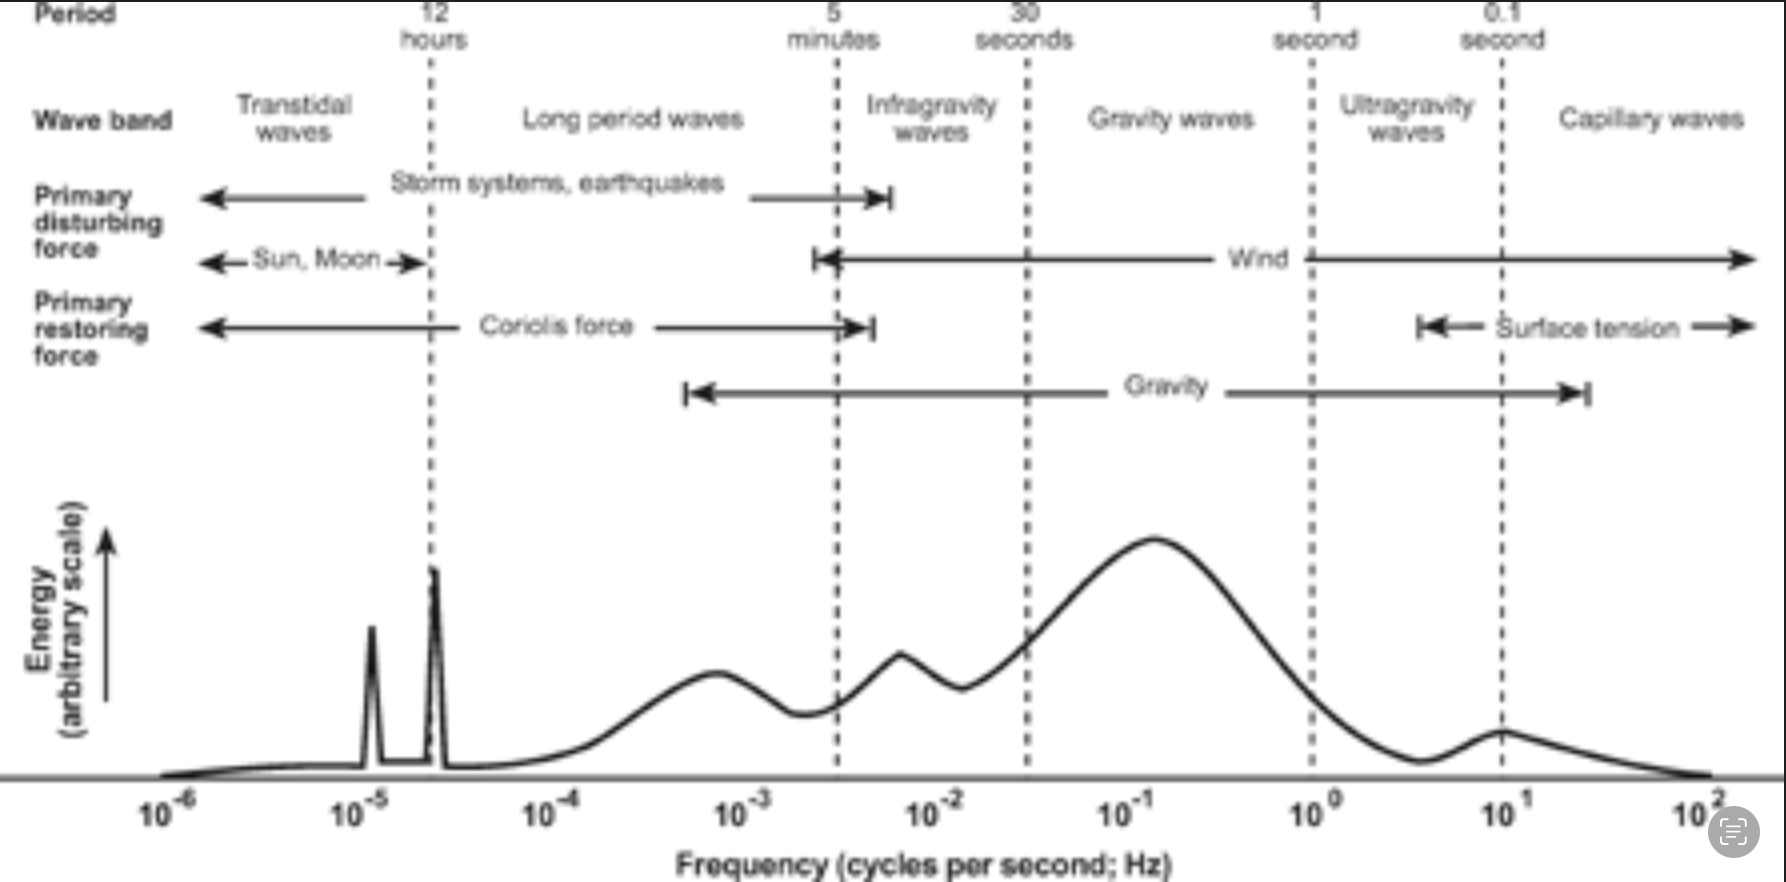
\includegraphics[width=1\linewidth]{images/ocean-wave-energy-schematic.png}
    \caption{Placeholder for self generated graphic based on this one from Kinsman, 1984\textsuperscript{[14]}}
    \label{figure2}
\end{figure}

\par{\hspace{.5cm}Ocean waves are created when a disturbing force acts on the ocean and a restoring force acts to restore equilibrium. These forces produce waves of varied frequency, wavelength, height, and direction.\textsuperscript{[6]}~\textsuperscript{[7]}~\textsuperscript{[11]}~\textsuperscript{[14]} The most commonly observable waves are wind waves: those generated by friction drag from wind blowing over an area of the ocean's surface, transferring energy into the to water.~\textsuperscript{[6]}~\textsuperscript{[7]}~\textsuperscript{[8]}~\textsuperscript{[9]}~\textsuperscript{[14]} A sea is area in which strong winds actively work to generate irregularly peaked waves of varied periodicity traveling in a broad spectrum of direction, resulting in a chaotic ocean surface. When energy losses from waves breaking are offset by energy gained from blowing wind, the sea is said to be fully developed or arisen.~\textsuperscript{[9]}~\textsuperscript{[14]}~\textsuperscript{[15]} The power spectra of a fully developed sea, first proposed by Willard Peirson and Lionel Moskowitz, is well defined, and allows forecasters to accurately model wave conditions based on wind speed and direction.~(\cref{figure3}).~\textsuperscript{[11]}~\textsuperscript{[15]}}

\par{To describe the processes by which wind generates waves more specifically, wind blowing over the ocean stretches the waters surface, and as surface tension works to restore it to equilibrium, capillary (low energy, short wavelength, high frequency) waves, are formed. As wind continues to blow, capillary waves are compounded by wind energy and grow. Capillary waves which exceed a wavelength threshold of 1.74cm become gravity waves, as gravity supersedes surface tension as the prevailing restoring force, and works to pull the crest of a wave downward. The water's inertia causes the crests to overshoot and become troughs, inducing a cycle in which water molecules oscillate in a near-frictionless orbit as gravitational forces work to restore the fluid to a state of equilibrium, allowing them to propagate long distances across the ocean's surface.~\textsuperscript{[6]}~\textsuperscript{[9]}~\textsuperscript{[11]} ~\textsuperscript{[14]} As wind activity ceases or waves move away from the area of generation, they are sorted into packets of uniform wavelength and direction. Gravity waves have a period around .1 Hz and represent the most energetic band of the spectra.~\textsuperscript{[6]}~\textsuperscript{[10]}~\textsuperscript{[11]}~\textsuperscript{[15]}.}

\begin{figure}
    \centering
    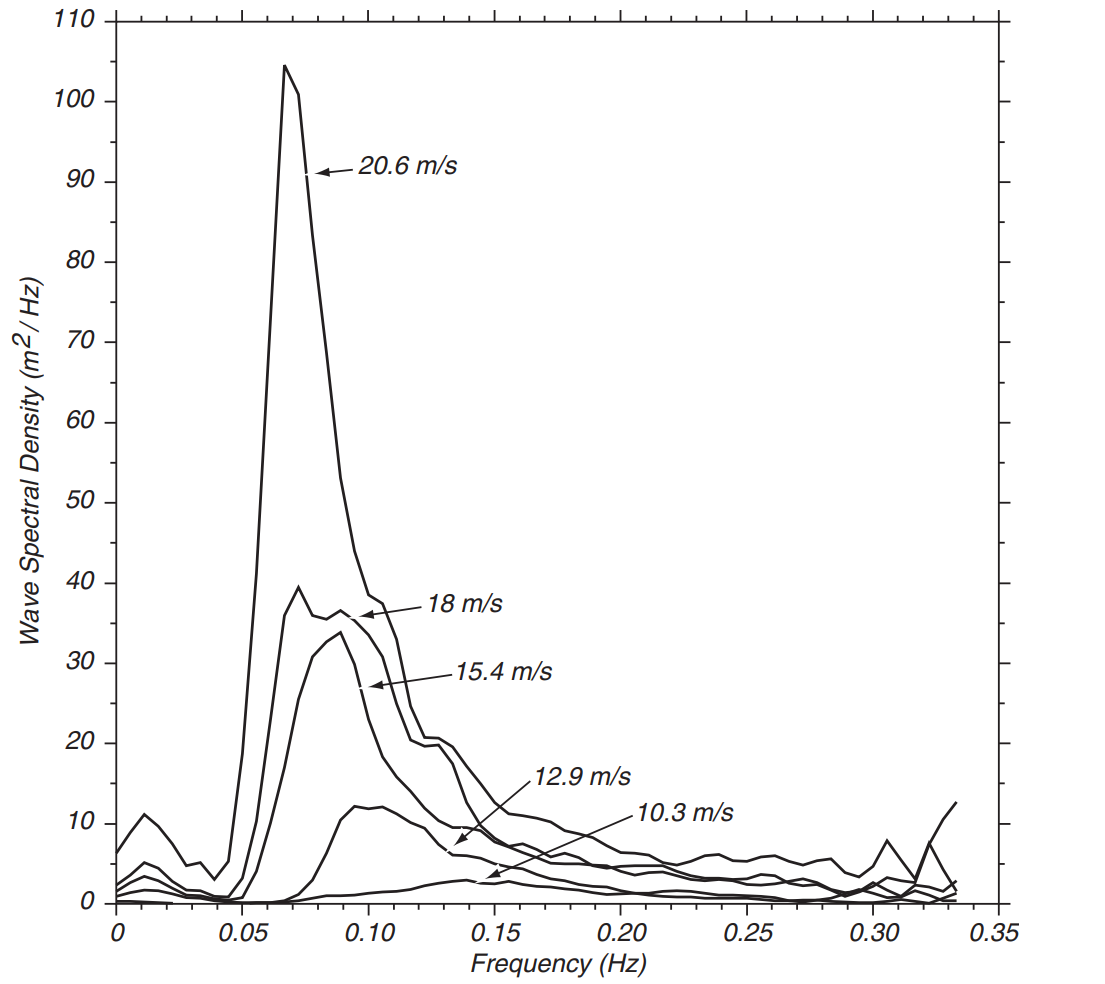
\includegraphics[width=0.75\linewidth]{images/developed-sea-power-spectrum.png}
    \captionof{figure}{Placeholder for self generated version of this Pierson-Moskowitz spectral graph.}
    \label{figure3}
\end{figure}
    
\par{All ocean waves propagate across the surface of the ocean as potential energy which is released as kinetic energy as they shoal through contact with bottom morphologies and are broken by spatial features of the nearshore zone and shoreface.~\textsuperscript{[6]}~\textsuperscript{[7]}~\textsuperscript{[9]} Gravity waves (10s) compound with phenomena occurring at longer time scales such as infragravity waves (30s - 300s), as well as tidal modulation and resulting instabilities from longshore currents (10\textsuperscript{2}-10\textsuperscript{3}-s), to create the full spectrum of nearshore gravity-based wave activity.~\textsuperscript{[7]}~\textsuperscript{[9]}~\textsuperscript{[12]}~\textsuperscript{[13]} Extreme events such as tsunamis generated by seismic activity and seiche (resonant rocking of water produced by sudden change in atmospheric pressure) may produce and augment nearshore wave activity episodically.~\textsuperscript{[7]}}

\par{Tides are another marine process that has a significant effect coastal areas, causing variation in sea level that augments wave activity and causes seawater to inundate and receed from low-lying areas, generating currents. The disturbing forces which generate tides are gravitational forces from the moon and sun which act on a rotating earth, causing global variation in local ocean surface height. Isaac Newton, in his work \textit{Principa Mathematica}, postulated the Equilibrium Theory of Tides, which described tides as two bulges of heightened sea level on opposite ends of the earth generated as the result of astrological forces acting upon the ocean's surface counter to earth's gravity.~\textsuperscript{[7]}~\textsuperscript{[9]}~\textsuperscript{[11]} Newton's theory was intentionally limited: it assumes infinitely deep oceans, not sufficient to explain how tidal wave height and length would exceed the extents of oceanic basins when considering the speed of solar and lunar positional change relative the earth.}

\par{Pierre-Simon Laplace expanded upon Newton's Equilibrium Theory of Tides by formulating the Dynamic Theory of Tides, which additionally incorporated phenomenon such as friction, the earth's rotation, the Coriolis effect, and the shape of oceanic basins, to more accurately characterize tidal behavior.~\textsuperscript{[7]}~\textsuperscript{[11]} The Dynamic Theory of Tides describes tidal waves that circulate about amphidromic points, where the tidal range is zero, counterclockwise in the Northern Hemisphere and clockwise in the Southern. Models incorporating these principles have been successful in predicting tides in accordance with observed behaviors.~\textsuperscript{[7]}~\textsuperscript{[11]}  When observed locally, tides are visible through the shoreline fluctuation between low and high tide once (diurnal) or twice (semidiurnal) daily depending on location relative to amphidromic points. These shifts generate longshore currents parallel to all coasts, and cross shore currents where tidal floods and ebbs rush into and out of enclosed areas such as estuaries and other inlets.~\textsuperscript{[7]}~\textsuperscript{[9]} In coastal areas sheltered from high wave energy, tidal activity can dominate local sediment transport, and exhibit significantly different physical and biological attributes from those predominantly effected by wave activity.~\textsuperscript{[11]}}

\begin{figure}
    \centering
    \includegraphics[width=0.75\linewidth]{images/eustatic-sea-level-change.png}
    \caption{Placeholder for self generated version of this graph from Chappell and Shackelton 1986.~\textsuperscript{[18]}}
    \label{figure4}
\end{figure}

\par{The most infrequent hydrodynamic processes which effect coastal waters are those associated with eustatic sea level change, or cumulative changes in the volume of the ocean from factors which occur over periods of 10\textsuperscript{5} years or longer, such as addition of water through glacial melting and volcanic out-gassing, thermal expansion of water, and changes in the shape of the seafloor through sediment deposit and tectonic spreading.~\textsuperscript{[4]}~\textsuperscript{[6]}~\textsuperscript{[17]} Local isostatic changes of land level with respect to sea height is caused by tectonic uplift from decadal lithospheric convergence.~\textsuperscript{[6]}~\textsuperscript{[17]} These processes have the most significant influence on shoreline change over longer timescales.~\textsuperscript{[4]} Sea levels have been continuously rising for the past \textasciitilde20,000 years since the Last Glacial Maximum (LGM), primarily caused by the melting of ice sheets from the Late Pleistocene, and is the primary contributor today's coastal and inland hydrological features, through inundation of low-lying continental areas and exposure of areas formally eroded and covered by glacial ice in high latitudes~\textsuperscript{[6]}~\textsuperscript{[8]}~\textsuperscript{[17]}~\textsuperscript{[18]}~\textsuperscript{[19]}}

\par{Watershed systems also work to influence coastal processes at areas where fresh water is channeled into an outlet and mix with oceanic salt water to form an estuary.~\textsuperscript{[9]}~\textsuperscript{[20]}~\textsuperscript{[21]}~\textsuperscript{[22]} At a rivermouth, the turbulent jetstream formed by fluvial discharge flowing into an estuary may dominate local hydrodynamics, the flow structure and velocity of which are dictated by the geometry of estuarine basin and are highly subject to episodic phenomenon such as storm surges or flooding events.~\textsuperscript{[20]}~\textsuperscript{[21]}~\textsuperscript{[22]} Where present, fluvial processes combine with tidal and wave action to form the overall hydrological gradient of that coastal locale, and may serve as the prevailing circulatory factor in some coastal areas which are well-sheltered from highly energetic marine processes.~\textsuperscript{[9]}~\textsuperscript{[20]}~\textsuperscript{[21]}~\textsuperscript{[22]}}

\subsection{Morphological}

\par{\hspace{.5cm}More nebulous than defining the coastal zone's extents are defining those of its sub-areas which group to form the full cross-shore (seaward normal from the shoreline) profile of a coast. Earlier, we adopted a definition of the coast as being an area where sub-decadal oceanic processes influence local morphology through sediment transport, and so we will divide the coastal zone into discrete sections based on which marine processes effect that area, and by extension the nature of sediment transport that occurs there. Therefore, by our definition, the furthest extent of a coast is the outer boundary where ocean waves shoal through contact with bottom morphologies. The offshore areas exceeding that boundary are unaffected by wave-action induced sediment transport and thus not included in our definition of the coastal zone.~\textsuperscript{[2]}~\textsuperscript{[6]}~\textsuperscript{[9]}~\textsuperscript{[16]}}

\begin{figure}
    \centering
    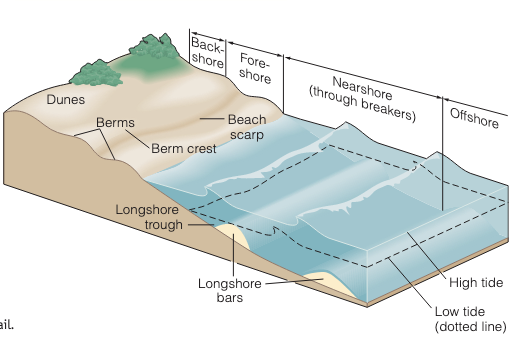
\includegraphics[width=1.0\linewidth]{images/coastal-sub-zones.png}
    \caption{Placeholder for self generated version of this infographic from Essentials of Oceanoraphy~\textsuperscript{[6]}}
    \label{figure5}
\end{figure}

\par{Adjacent to that and proximal to the shoreline, is the littoral zone, the greater area in which sediment transport occurs both on in the water and on land.~\textsuperscript{[8]}~\textsuperscript{[16]} The littoral zone can be divided further into the nearshore, foreshore, and backshore areas~(\cref{figure5}). The seaward limit of the nearshore is the offshore boundary and extends to the shoreline. At the offshore boundary, waves shoal as depth becomes half the wavelength of incident wave, and break as they come into further contact with bottom morphologies in the surf zone, also included as a subsection of the nearshore. The foreshore is the section landward from the shoreline and extending to the high-high-water (HHW) mark, the extent to which the combination of tidal and wave activity reach.~\textsuperscript{[16]} Continuing landward, the backshore area begins at the HHW to the end of where loose sediment particles are deposited. Sediment in the backshore is subject mostly to daily aeolian transport, but can also be effected by episodic extreme wave and surge action from storms.~\textsuperscript{[2]}~\textsuperscript{[9]}~\textsuperscript{[12]}~\textsuperscript{[16]}}

\begin{figure}
    \centering
    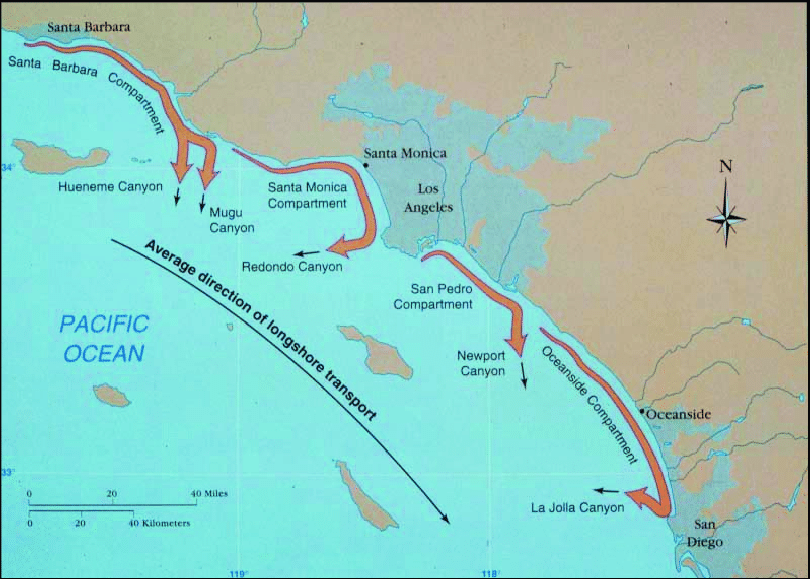
\includegraphics[width=.9\linewidth]{images/so-cal-littoral-cells.png}
    \caption{Placeholder for self generated version of this infographic from Littoral Cells in Southern California by Inman and Chamberlain ~\textsuperscript{[24]}}
    \label{figure6}
\end{figure}

\par{Sedimentary charactertistics serve as a useful basis for classification schemes for coasts. One important distinction is between areas of coast which regularly experience a net gain in sediment accumulation as opposed to those which experience a net loss, cateogrized as either depositional and erosional respectively. Another distinction can be made based on the size of sediment grains present onshore, which ranges on a continuum from cliffs and large boulders, to rocks, to sand, to fine-grain mud.~\textsuperscript{[23]} Environments with different sedimentary characteristics exhibit vastly different geomorphic and biotic traits. Sedimentary characteristics are strongly correlated with energy from wave action: often coasts exposed to areas of high wave activity are erosional, as sediment becomes dislodged by wave energy and is transported by currents until it becomes deposited at sheltered beaches nearby.~\textsuperscript{[9]} The geometry of the littoral area also plays a factor: steepness and size of the foreshore and bathymetric gradients in the nearshore correlate to erosional rates and grain size. ~\textsuperscript{[8]}~\textsuperscript{[9]}~\textsuperscript{[16]}~\textsuperscript{[23]}}

\par{Segmenting coastlines according to sediment transport characteristics is also highly pertinent. A coastal or littoral cell is a contiguous sector of coastline in which erosional and accretionary processes are balanced, and spans the distance sediment is transported from an erosional source to the extent to which it is largely deposited or lost offshore.~(\cref{figure6}).~\textsuperscript{[9]}~\textsuperscript{[16]} The recognition of discrete littoral cells is essential to understanding and characterizing coastal morphological processes, and is regularly used as a tool in coastal land management and development.~\textsuperscript{[23]} Often littoral cells are bordered by clear geographic markers, such as headlands which restrict the angle of wave approach to the shoreline to disrupt the flow of sediment, and submarine canyons which channel sediments offshore.~\textsuperscript{[23]}~\textsuperscript{[24]} \par}

\par{A littoral cell experiences net transport of sediment in a single direction parallel to the shore.~\textsuperscript{[6]}~\textsuperscript{[16]} Waves refract in shallow water to break near-parallel to shore, but maintain a slight angle as they crash on the shoreface, resulting in Swash, a turbulent layer of onshore water.~\textsuperscript{[6]}~\textsuperscript{[28]} Swash rushes up the beach up at the angle of the breaking wave, then retreats straight down towards the shoreline due to gravity, during phases refered to as uprush and backwash respectively.~\textsuperscript{[6]}~\textsuperscript{[28]} Through uprush and backwash, sediment is loosened and then transported in a zig-zag pattern up and down the beach, with net direction parallel to the coast, in a collective process known as longshore drift.~\textsuperscript{[6]}~\textsuperscript{[28]} Local properties such as geographic location, shoreline irregularities, nearshore geometry, wind and wave energy, tidal currents, and sediment size, compound to influence how much sediment is removed, how quickly and in which direction sediment is transported, and where it becomes deposited.~\textsuperscript{[6]}~\textsuperscript{[8]}~\textsuperscript{[12]}~\textsuperscript{[16]}~\textsuperscript{[28]} Sediment will be continuously deposited and transported longshore until the drift is interrupted or diverted by shoreline irregularities at the end of a littoral cell.~\textsuperscript{[24]}}

\begin{figure}
    \centering
    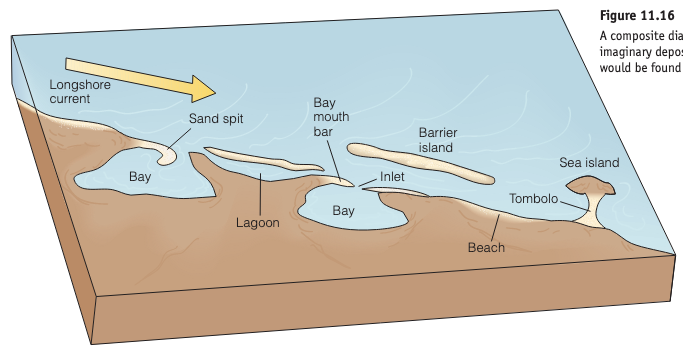
\includegraphics[width=.9\linewidth]{images/coastal-morphology.png}
    \caption{Placeholder for self generated version of this infographic from Essentials of Oceanography ~\textsuperscript{[6]}}
    \label{figure7}
\end{figure}

\par{Coastal morphologies in the nearshore and foreshore are formed when sediment is removed or deposited as a result of hydrodynamic processes occuring over time, and so erosional coasts exhibit a different array of morphological features from depositional ones. Net sediment loss at erosional coasts expose bedrock directly to wave action. Waves erode bedrock by pushing air and water into small fissures which build pressure to fracture and dislodge debris. Additionally, waves may hurl debris, and water from waves may dissolve minerals in certain types of rock to contribute to erosion more effectively.~\textsuperscript{[6]} Erosion occurs mostly at the water line, so the bedrock may develop at notches at the water line.~\textsuperscript{[6]}~\textsuperscript{[16]}~\textsuperscript{[28]} Notching can cause the rock above to collapse to form a steep cliff, and may result in other formations, as weaker zones of bedrock are removed to form features within the cliff-side such as caves. The base of notches into a cliff-side at the low tide mark which may remain as the ceiling above collapses, leaving a large flat wave-cut platform of rock at the low-tide line which remains submerged and unaffected during higher tides Formations such as sea stacks and arches may remain beyond the shoreline as the weaker rock around them is removed.~\textsuperscript{[6]} Longshore currents transport sediment generated through these erosive processes until it is deposited in more sheltered areas such as nearby bays, or removed.~\textsuperscript{[6]}~\textsuperscript{[28]} }

\par{Fluvial systems are the primary input for sediment into the coastal area, as loose soil particles derived mostly from rain-based erosion are transported downstream and into estuaries.~\textsuperscript{[8]}~\textsuperscript{[20]}~\textsuperscript{[23]}~\textsuperscript{[25]} In areas subject to high wave activity, sediment removed by wave action may exceed sediment deposited from fluvial processes, resulting in erosion.~\textsuperscript{[20]}~\textsuperscript{[26]} Tidal intrusion into estuaries creates currents which interact with jetsteams at the river-mouth and may create shear fronts and other complex flows which result in unique morphologies.~\textsuperscript{[6]}~\textsuperscript{[8]}~\textsuperscript{[27]} Watershed areas with low wave and tidal activity are more likely to experience sediment accumulation, which may result in depositional landforms such as deltas which penetrate into coastal waters.~\textsuperscript{[6]}~\textsuperscript{[8]}~\textsuperscript{[16]} Anthropic manipulation of watershed systems can also have a significant impact on fluvial sediment transport and deposition, as damming, dredging, and other forms of water management can alter the natural flow of sediment downstream.~\textsuperscript{[16]}~\textsuperscript{[26]}}

\par{Most familiarly depositional coasts develop beaches, which is a zone of loose particles that covers the shore.~\textsuperscript{[6]} Beach particles may be generated from different sources—--many are generated from the processes described earlier, such as cliff erosion and fluvial discharge, but others in tropical regions are composed of biological particles such shells and fragments of coral, and in regions subject to volcanic activity may be composed to fragments of andesite or basalt from lava.~\textsuperscript{[6]}~\textsuperscript{[16]}~\textsuperscript{[26]} Particles can range in size from silt (0.0039-0.0625mm), to sand (0.0625-2mm), to pebbles and cobbles (0.5-256mm), to boulders (greater than 256mm), determined primarily by three factors: sediment source, wave-energy level, and offshore slope upon which the beach is constructed.~\textsuperscript{[26]} A single beach is composed of grains of many different sizes which become sorted through wave action, creating a strong correlation between mean grain size and wave energy level both up and offshore.~\textsuperscript{[26]} Beaches develop distinguishable morphologies induced by the marine processes to which they're exposed on their faces---the extent of wave and tidal action often creates a accumulation of sediment parallel to the shoreline called a berm, which marks the boundary between the fore and backshore areas.~\textsuperscript{[6]}~\textsuperscript{[26]}. Scarps are formed at the same boundary, but instead when erosional wave action removes sediment to form a steep cliff.~\textsuperscript{[6]}~\textsuperscript{[26]}~\textsuperscript{[30]} Landward from that boundary, the backshore area may form dunes. }

\par{emergent barrier systems of landforms seperated from the mainland by a lagoon, bay, or marsh, which are formed when sediment particles become deposted onto an subaqueous platform or base. 

\par{Another common feature of depositional coasts are longshore bars.}


\par{Many aquatic coastal features were formed as a result of eustatic sea level rise caused by the melting of glaciers since the LGM, which flooded low-lying continental areas such as river valleys.~\textsuperscript{[6]}~\textsuperscript{[8]} These features may be categorized according to the influence of different hydrodynamic processes in their formation and composition. Bays are larger bodies of water partially enclosed by land, and can be either fully open to the ocean or partially sheltered by landforms. Lagoons are shallow bodies of salt water that have become partially or fully enclosed by the development of accumulation of sediments into a barrier, or by biological barriers such as reefs, which largely shields them from marine processes.}

\par{Estuaries are often at the focus of coastal sciences, as they represent some of the most highly dynamic and productive coastal environments. They are generally sheltered from wave action, but may be subject to daily tidal inundation and recession of varying degrees. Estuarine bodies beg further sub-classification, as they can range drastically according to their expoisure to disparate hydrodynamic processes, which in turn dictates how they're formed, as well as the daily fluctuation of their composition. In mountaneous areas of higher latitudes, glaciers formed during the Pleistocene eroded valleys into deep u-shaped troughs, and have since retreaded to create fjords, long narrow marine inlets with steep sides.}

\begin{figure}
    \centering
    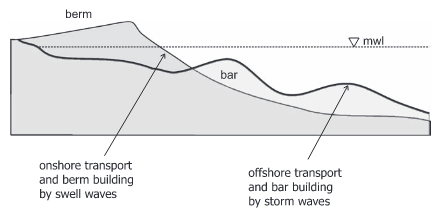
\includegraphics[width=.9\linewidth]{images/barred-profile.png}
    \caption{Placeholder for self generated version of this infographic from Introduction to Coastal Processes and Geomorphology} ~\textsuperscript{[16]}
    \label{figure8}
\end{figure}



\par{**Biological effects on morphology: reefs, mangroves, salt flats, etc...**}

\par{**Other factors: volcanism, plate tectonics, glaciers**}

\par{**Geographical effects on erosional / depositional: Trialing edge, roaring 40s, etc...**}

% REFERENCE
\newpage
\fancyhead[C]{REFERENCE}
\fancyfoot[C]{\thepage} 
\thispagestyle{fancy}
\section{Reference}

\begin{enumerate}

    \item {“NOAA’s National Weather Service - Glossary.” Accessed: May 01, 2025. [Online]. \href{https://forecast.weather.gov/glossary.php?word=coastal%20waters}{Available}}
    
    \item {“Definition of the coast,” Geosciences LibreTexts. Accessed: May 01, 2025. [Online]. \href{https://geo.libretexts.org/Bookshelves/Oceanography/Coastal_Dynamics_(Bosboom_and_Stive)/01%3A_Overview/1.05%3A_Coastal_(morpho)_dynamics/1.5.01%3A_Definition_of_the_coast}{Available}}
    
    \item {“Comparative analysis II: Land demarcation and property rights,” in ResearchGate. Accessed: May 04, 2025. [Online]. \href{https://www.researchgate.net/publication/362949604_Comparative_analysis_II_Land_demarcation_and_property_rights}{Available}}
    
    \item {E. Hunt, M. Davidson, E. C. C. Steele, J. D. Amies, T. Scott, and P. Russell, “Shoreline modelling on timescales of days to decades,” Cambridge Prisms: Coastal Futures, vol. 1, p. e16, Jan. 2023, doi: 10.1017/cft.2023.5.}

    \item {M. A. Davidson, K. D. Splinter, and I. L. Turner, “A simple equilibrium model for predicting shoreline change,” Coastal Engineering, vol. 73, pp. 191–202, Mar. 2013, doi: 10.1016/j.coastaleng.2012.11.002.}

    \item {T. Garrison, Essentials of oceanography, 6th ed. Belmont, CA: Brooks/Cole, Cengage Learning, 2012.}

    \item {R. Holman and M. C. Haller, “Remote Sensing of the Nearshore,” Annu. Rev. Mar. Sci., vol. 5, no. 1, pp. 95–113, Jan. 2013, doi: 10.1146/annurev-marine-121211-172408.}

    \item {M. J. Kaiser and P. J. leB Williams, Eds., Marine ecology: processes, systems, and impacts, 2nd ed. Oxford; New York: Oxford University Press, 2011.}

    \item {“Coastal Processes and Beaches | Learn Science at Scitable.” Accessed: May 05, 2025. [Online]. \href{https://www.nature.com/scitable/knowledge/library/coastal-processes-and-beaches-26276621/}{Available}}

    \item {N. US Department of Commerce, “Marine Definitions.” Accessed: May 06, 2025. [Online]. \href{https://www.weather.gov/gum/MarineDefinitions}{Available}}

    \item {G. Masselink, Introduction to coastal processes and geomorphology, Second edition. Oxon [England]: Routledge, 2014. doi: 10.4324/9780203785461.}

    \item {E. B. Thornton and C. S. Kim, “Longshore current and wave height modulation at tidal frequency inside the surf zone,” Journal of Geophysical Research: Oceans, vol. 98, no. C9, pp. 16509–16519, 1993, doi: 10.1029/93JC01440.}

    \item {T. C. Lippmann, A. H. Brookins, and E. B. Thornton, “Wave energy transformation on natural profiles,” Coastal Engineering, vol. 27, no. 1, pp. 1–20, May 1996, doi: 10.1016/0378-3839(95)00036-4.}

    \item {B. Kinsman, Wind Waves: Their Generation and Propagation on the Ocean Surface. New York: Dover Publications, 1984.}

    \item {W. J. Pierson Jr. and L. Moskowitz, “A proposed spectral form for fully developed wind seas based on the similarity theory of S. A. Kitaigorodskii,” Journal of Geophysical Research (1896-1977), vol. 69, no. 24, pp. 5181–5190, 1964, doi: 10.1029/JZ069i024p05181.}

    \item {R. Davidson-Arnott, “An Introduction to Coastal Processes and Geomorphology”.}

    \item {K. Fleming, P. Johnston, D. Zwartz, Y. Yokoyama, K. Lambeck, and J. Chappell, “Refining the eustatic sea-level curve since the Last Glacial Maximum using far- and intermediate-field sites,” Earth and Planetary Science Letters, vol. 163, no. 1, pp. 327–342, Nov. 1998, doi: 10.1016/S0012-821X(98)00198-8.}

    \item {“Coastal prehistory in the southern Red Sea Basin, underwater archaeology, and the Farasan Islands,” ResearchGate. Accessed: May 08, 2025. [Online]. \href{https://www.researchgate.net/publication/277182725_Coastal_prehistory_in_the_southern_Red_Sea_Basin_underwater_archaeology_and_the_Farasan_Islands}{Available}}

    \item {"N. J. Shackleton, “Oxygen isotopes, ice volume and sea level,” Quaternary Science Reviews, vol. 6, no. 3–4, pp. 183–190, Jan. 1987, doi: 10.1016/0277-3791(87)90003-5."}

    \item {"H. Ji, S. Pan, and S. Chen, “Impact of river discharge on hydrodynamics and sedimentary processes at Yellow River Delta,” Marine Geology, vol. 425, p. 106210, Jul. 2020, doi: 10.1016/j.margeo.2020.106210."}

    \item{"C. M. Broaddus et al., “First‐Order River Delta Morphology Is Explained by the Sediment Flux Balance From Rivers, Waves, and Tides,” Geophysical Research Letters, vol. 49, no. 22, p. e2022GL100355, Nov. 2022, doi: 10.1029/2022GL100355."}

    \item{A. Ruiz-Reina, A. López-Ruiz, and M. Ortega-Sánchez, “River Mouth Hydrodynamics: The Role of the Outlet Geometry and Transient Tidal and River Discharge Conditions on the Jet Structure,” Journal of Geophysical Research: Oceans, vol. 130, no. 1, p. e2024JC021500, 2025, doi: 10.1029/2024JC021500.}

    \item{K. Patsch and G. Griggs, “DEVELOPMENT OF SAND BUDGETS FOR CALIFORNIA S MAJOR LITTORAL CELLS”.}

    \item{Littoral cells in Southern California. (Inman and Chamberlain, 1960) Accessed: May 11, 2025. [Online] \href{https://www.researchgate.net/figure/Littoral-cells-in-Southern-California-Inman-and-Chamberlain-1960-Thurman-and_fig4_240635473}{Available}}

    \item{M. M. Alemu, “Integrated Watershed Management and Sedimentation,” Journal of Environmental Protection, vol. 7, no. 4, Art. no. 4, Mar. 2016, doi: 10.4236/jep.2016.74043.}

    \item{A. W. Stevens et al., “Monitoring and modeling dispersal of a submerged nearshore berm at the mouth of the Columbia River, USA,” Coastal Engineering, vol. 181, p. 104285, Apr. 2023, doi: 10.1016/j.coastaleng.2023.104285.}

    \item{W. R. Geyer, D. K. Ralston, M. C. Haller, C. Bassett, and D. Honegger, “The Structure and Dynamics of an Estuarine Tidal Intrusion Front,” Journal of Geophysical Research: Oceans, vol. 129, no. 2, p. e2023JC020371, 2024, doi: 10.1029/2023JC020371.}

    \item{P. D. Komar, Beach processes and sedimentation. Upper Saddle River, N.J.: Prentice Hall, 1998. Accessed: May 15, 2025. [Online]. \href{http://archive.org/details/beachprocessesse0002koma}{Available}}

    \item{[T. J. O’Hare and D. A. Huntley, “Bar formation due to wave groups and associated long waves,” Marine Geology, vol. 116, no. 3–4, pp. 313–325, Feb. 1994, doi: 10.1016/0025-3227(94)90048-5.}

    \item{C. W. T. van Bemmelen, M. A. de Schipper, J. Darnall, and S. G. J. Aarninkhof, “Beach scarp dynamics at nourished beaches,” Coastal Engineering, vol. 160, p. 103725, Sep. 2020, doi: 10.1016/j.coastaleng.2020.103725.}


    }

\end{enumerate}

% END DOCUMENT
\end{document}